% ============================================================================
%  SP1 Phase-1 Report — AI-Enabled Smart EV Charging and Energy Management
%  Compiled with xelatex (see docs/README or the workspace report rules).
%
%  Build:
%     cd docs/phase1-report
%     xelatex phase1-report.tex
%     xelatex phase1-report.tex        % twice, so \ref / \cite settle
% ============================================================================
\documentclass[11pt,a4paper]{article}

% --- encoding & fonts -------------------------------------------------------
\usepackage[UTF8]{ctex}          % CJK support (works with xelatex)
\usepackage{fontspec}
\setmainfont{Times New Roman}
\setsansfont{Arial}
\setmonofont{Consolas}

% --- layout & typography ----------------------------------------------------
\usepackage[a4paper,margin=2.4cm]{geometry}
\usepackage{graphicx}
\usepackage{float}
\usepackage{booktabs}
\usepackage{longtable}
\usepackage{array}
\usepackage{amsmath}
\usepackage{xcolor}
\usepackage{enumitem}
\usepackage{caption}
\usepackage{fancyhdr}
\usepackage[hidelinks]{hyperref}
\usepackage{parskip}

% --- overflow prevention ----------------------------------------------------
\usepackage[htt]{hyphenat}
\setlength{\emergencystretch}{2.5em}

\captionsetup{font=small,labelfont=bf}
\graphicspath{{figures/}}
\setlist[itemize]{leftmargin=1.4em,topsep=2pt,itemsep=2pt}
\setlist[enumerate]{leftmargin=1.6em,topsep=2pt,itemsep=2pt}

\renewcommand{\topfraction}{0.92}
\renewcommand{\bottomfraction}{0.85}
\renewcommand{\textfraction}{0.06}
\renewcommand{\floatpagefraction}{0.85}

\pagestyle{fancy}
\fancyhf{}
\fancyhead[L]{\small FYP — Smart EV Charging Platform}
\fancyhead[R]{\small SP1 Phase-1 Report}
\fancyfoot[C]{\small\thepage}
\renewcommand{\headrulewidth}{0.4pt}

\newcommand{\code}[1]{\texttt{\small #1}}

% Numbers quoted in the text and in the results tables. Generated from the pipeline artefacts by
% scripts/make_report_tables.py — the single source of truth, never hand-copied.
% generated by scripts/make_report_tables.py -- do not edit by hand
\newcommand{\BoulderOrigins}{25}
\newcommand{\BoulderIntervals}{600}
\newcommand{\BoulderBest}{gradient boosting}
\newcommand{\BoulderWape}{0.292}
\newcommand{\BoulderRtwo}{0.763}
\newcommand{\BoulderNaiveWape}{0.360}
\newcommand{\BoulderImprovement}{19}
\newcommand{\PaloAltoOrigins}{14}
\newcommand{\PaloAltoIntervals}{336}
\newcommand{\PaloAltoWape}{0.549}
\newcommand{\PaloAltoNaiveWape}{0.670}
\newcommand{\PaloAltoImprovement}{18}
\newcommand{\WindowHours}{600}
\newcommand{\ForecastPeak}{94.5}
\newcommand{\BaselinePeak}{362.5}
\newcommand{\PeakAmplification}{3.8}
\newcommand{\BiasPct}{+3.5}
\newcommand{\ConservedPct}{+0.05}
\newcommand{\CoveragePct}{91.0}
\newcommand{\ForecastMwh}{17.81}
\newcommand{\BaselineMwh}{17.22}
\newcommand{\ActualMwh}{17.21}
\newcommand{\IntervalWidth}{33.2}
\newcommand{\BoulderGwh}{1.253}
\newcommand{\BoulderPeakHour}{11:00}
\newcommand{\BoulderPeakShare}{8.2}
\newcommand{\BoulderTroughHour}{04:00}
\newcommand{\BoulderTroughShare}{0.42}
\newcommand{\BoulderRatio}{19.3}
\newcommand{\PaloAltoGwh}{2.216}
\newcommand{\PaloAltoPeakHour}{12:00}
\newcommand{\PaloAltoPeakShare}{7.9}
\newcommand{\PaloAltoTroughHour}{04:00}
\newcommand{\PaloAltoTroughShare}{0.41}
\newcommand{\PaloAltoRatio}{19.2}


% ============================================================================
\begin{document}

\begin{center}
  {\LARGE\bfseries AI-Enabled Smart Electric Vehicle Charging\\[2pt]
   and Energy Management Platform}\\[8pt]
  {\large\bfseries Sub-Project 1 — Phase 1 Report}\\[4pt]
  {\large Data acquisition, preprocessing and demand-forecasting baseline}
\end{center}

\begin{table}[H]
\centering
\begin{tabular}{@{}ll@{}}
\toprule
Sub-project & SP1 — EV charging data analysis and demand forecasting \\
Owner      & Xu Yuxuan \\
Supervisor & Dr Amer Ghias (University of Glasgow / Glasgow College UESTC) \\
Date       & 14 September 2026 \\
\midrule
Deliverables covered & Clean datasets; analysis framework; forecasting models; accuracy evaluation \\
Code        & \code{subprojects/sp1-data-forecasting/} \\
Outputs     & \code{data/processed/sp1-demand-forecast-v1.csv} \\
            & \code{data/processed/sp1-baseline-demand-v1.csv} \\
\bottomrule
\end{tabular}
\end{table}

% ============================================================================
\section{Scope and objectives}

SP1 owns the first stage of the platform's data flow: it turns raw public charging
records into the gap-free hourly demand series that every other sub-project consumes
(SP2 schedules against it, SP4 displays it, SP5 prices it). The official brief assigns
SP1 four tasks: collect and preprocess public EV charging datasets; analyse charging
patterns and user behaviour; develop machine-learning models to predict future charging
demand; and evaluate forecasting accuracy and model performance. This report covers all
four, and with them the Phase-1 milestone (datasets secured, tools aligned, framework
running).

Two constraints shaped the work and are resolved in Section~\ref{sec:data}:

\begin{enumerate}
  \item \textbf{Dataset selection.} The supervisor's kickoff email named three sources — Caltech
        ACN-Data, Boulder Colorado, and UK National Grid — and each was checked against its live
        service. The outcome decided the project's data foundation.
  \item \textbf{Official provenance.} The earlier plan assumed Chinese datasets. A member-account
        review of the China Charging Alliance platform and a search of provincial and
        grid-operator portals found no session-level Chinese data, so that route could not carry a
        forecasting model.
\end{enumerate}

% ============================================================================
\section{Data acquisition and source evaluation}\label{sec:data}

\subsection{Sources verified}

Every source below was probed with live requests (HTTP status, schema, row counts, licence
text); nothing is quoted from a landing page without having been observed. The full
verification log is kept in the repository at \code{data/raw/official-datasets-research.md}.

\begin{table}[H]
\centering
\resizebox{\textwidth}{!}{%
\begin{tabular}{@{}p{3.5cm}p{2.2cm}p{2.6cm}p{4.0cm}p{3.1cm}@{}}
\toprule
Source & Official? & EV charging data? & Access observed & Verdict \\
\midrule
City of Boulder, Colorado & Yes — municipal government & Yes — sessions, metered kWh & ArcGIS FeatureServer, no registration; 148{,}136 rows pulled & \textbf{In use (primary)} CC0 1.0 \\
City of Palo Alto, California & Yes — municipal government & Yes — sessions, metered kWh, user IDs & Direct CSV, no registration; 85.4\,MB, 259{,}415 rows & \textbf{In use (validation)} PDDL \\
Caltech ACN-Data & Yes — Caltech + PowerFlex & Yes — sessions \emph{plus} measured power time series & API returns HTTP 401; free self-registration issues a token & Obtainable; not used yet (see \S\ref{sec:next}) \\
UK National Grid (now NESO) & Yes — national system operator & \textbf{No} — GB national demand only & CKAN/CSV, no registration, 2001--2025 & Not an EV dataset; grid context only \\
China Charging Alliance & Yes — industry alliance & \textbf{No} — monthly aggregates only & Member account required & Could not support SP1 \\
\bottomrule
\end{tabular}%
}
\caption{Sources checked for SP1. Only the first two provide session-level EV charging records that are official \emph{and} downloadable without a signed agreement.}
\label{tab:sources}
\end{table}

Two consequences follow, and both are recorded in the integration contract as
amendment~A1 rather than being decided quietly:

\begin{itemize}
  \item \textbf{Region.} The project can no longer be described as China-only; the demand
        series is for two US cities. The file formats are unchanged.
  \item \textbf{Currency.} Neither dataset contains a tariff or price column, so CNY pricing
        has no basis. SP2 must source a US tariff schedule before it can populate
        \code{tariff\_cny\_per\_kwh}; that is now an open item owned by SP2.
\end{itemize}

\subsection{Datasets used}

\begin{table}[H]
\centering
\resizebox{\textwidth}{!}{%
\begin{tabular}{@{}lrr@{}}
\toprule
Property & City of Boulder (primary) & City of Palo Alto (validation) \\
\midrule
Publisher & City of Boulder Open Data & City of Palo Alto Open Data \\
Licence & CC0 1.0 (public domain) & PDDL (public domain) \\
Sessions & 148{,}136 & 259{,}415 \\
Stations & 50 (all Level 2) & 47 \\
Period & 2018-01-02 -- 2023-12-01 (5.9 years) & 2011-07-30 -- 2021-01-01 (9.4 years) \\
Energy column & \code{Energy (kWh)} — \textbf{metered} & \code{Energy (kWh)} — \textbf{metered} \\
Timestamps & start and end, minute resolution & start and end, minute resolution \\
Per-vehicle ID & none & \code{User ID}, 97\% populated \\
Hourly series & \emph{derived} (see \S\ref{sec:method}) & \emph{derived} \\
Rows with zero energy & 16{,}113 (10.9\%) & --- \\
\bottomrule
\end{tabular}%
}
\caption{The two datasets actually used. Both are ChargePoint-style exports, so both
share the same traps, handled below.}
\label{tab:datasets}
\end{table}

\subsection{Cleaning decisions}

The datasets are published as session records, so ``cleaning'' here means mapping them into
one canonical schema and refusing to let known traps through silently.

\begin{enumerate}
  \item \textbf{Occupancy and charging time.} Both sources publish a total plugged-in
        duration \emph{and} an active charging duration. In Boulder the median occupancy is
        1.55\,h but the tail reaches 839\,h (vehicles left connected for weeks). Spreading a
        session's energy across occupancy would smear the load profile into nonsense, so the
        adapter maps the canonical duration to \emph{charging} time (median 1.39\,h,
        99th percentile 8.3\,h) and defines the session window as
        \code{start}~$\rightarrow$~\code{start + charging\_time}.
  \item \textbf{Units and types.} Boulder delivers every column as a string, including
        numerics; the adapter casts explicitly and reports unparsable values instead of
        dropping rows. Durations arrive as \code{hh:mm:ss} rather than minutes, which the
        adapter now parses in either form.
  \item \textbf{Timezone.} Storage is UTC. Source timestamps are naive local time; each
        dataset declares its own zone (\code{America/Denver}, \code{America/Los\_Angeles}) and
        is converted on load, so daylight saving is handled by the timezone database rather
        than by the file's own (sometimes inconsistent) zone label.
  \item \textbf{Energy provenance.} These datasets measure delivered energy. Where a dataset
        instead publishes only a \emph{rated} power, energy becomes a derived upper bound;
        that is a materially weaker input and was one reason the Chinese third-party dataset
        was set aside.
\end{enumerate}

% ============================================================================
\section{Method}\label{sec:method}

\subsection{From sessions to an hourly demand series}

Each session contributes its metered energy to every hourly interval it overlaps, in
proportion to the overlap duration. The result is energy per interval, which at a
one-hour resolution is numerically the average power in kW. Absent intervals mean ``no
charging recorded'', which for demand is a true zero, so the grid is completed with zeros;
the contract's guarantee to downstream sub-projects is a \emph{gap-free, non-negative,
UTC-stamped} series, and the pipeline re-reads and validates every file it writes.

One modelling assumption applies throughout: the datasets contain no intra-session power trace, so
a session's energy is spread \emph{evenly} across its charging window. Real charging curves taper,
so this slightly smooths peaks within a session. The assumption is recorded in each output's
\code{.meta.json} under \code{interval\_method}, so no downstream sub-project has to infer it.

\subsection{The uncontrolled baseline}

SP2 and SP5 need something to compare an optimised schedule against, so SP1 also emits an
``uncontrolled'' profile: every session's energy is moved to a block starting at 18:00 local
on the day it occurred, charged at that session's own recorded power. Energy is therefore
conserved and only its timing changes — a deliberate worst-case shape, not a network
simulation. (At a fixed 7\,kW this would stretch a 150\,kW fast-charge session over 40 hours;
using each session's own power avoids that artefact.)

\subsection{Features and forecasting}

Forecasting is framed as \emph{direct multi-horizon forecasting with the horizon as a
feature}: one model predicts all 24 hours from a single origin, so errors do not accumulate
the way they do in recursive one-step prediction.

\begin{itemize}
  \item \textbf{Known-future features} describe the \emph{target} interval: local hour of
        day, day of week, weekend flag, month, and cyclical encodings. These are known in
        advance, so using them is legitimate.
  \item \textbf{Autoregressive features} describe the \emph{origin}: demand lags of 1, 2, 3,
        24, 48 and 168 hours and rolling means, standard deviations and maxima over 24 and
        168 hours, all shifted so they cannot see the interval being predicted.
  \item \textbf{Naive references} are first-class inputs: the value 24 hours and 168 hours
        before the target, which also serve as the persistence baselines.
\end{itemize}

A regression test recomputes every lag from the raw series and fails if any feature can see
its own target; a second one pins the training boundary with a ramp series, because a leaky
backtest reports fantasy accuracy.

\subsection{Models and evaluation}

Seven models are scored: three baselines (\code{naive\_daily}, \code{naive\_weekly},
\code{hour\_of\_week\_profile}) and four learned models (ridge regression, random forest,
gradient boosting, XGBoost). Evaluation uses a rolling-origin backtest: for each
origin the model is retrained using only targets strictly before that origin, and forecasts
the next 24 hours. Origins are anchored to local midnight, so each is a genuine day-ahead
forecast, and only origins with a full horizon are used, which keeps the evaluation window
gap-free. Training history per origin is capped at 180 days.

Accuracy is reported as WAPE (total absolute error divided by total demand), which
stays stable when many intervals have near-zero demand, alongside MAE, RMSE and $R^2$.
Confidence bounds are empirical: $\hat{y} \pm 1.645\,\sigma$ where $\sigma$ is the residual
standard deviation at the same horizon in the backtest, clipped at zero.

% ============================================================================
\section{Results}\label{sec:results}

\subsection{Charging patterns}

\begin{figure}[H]
  \centering
  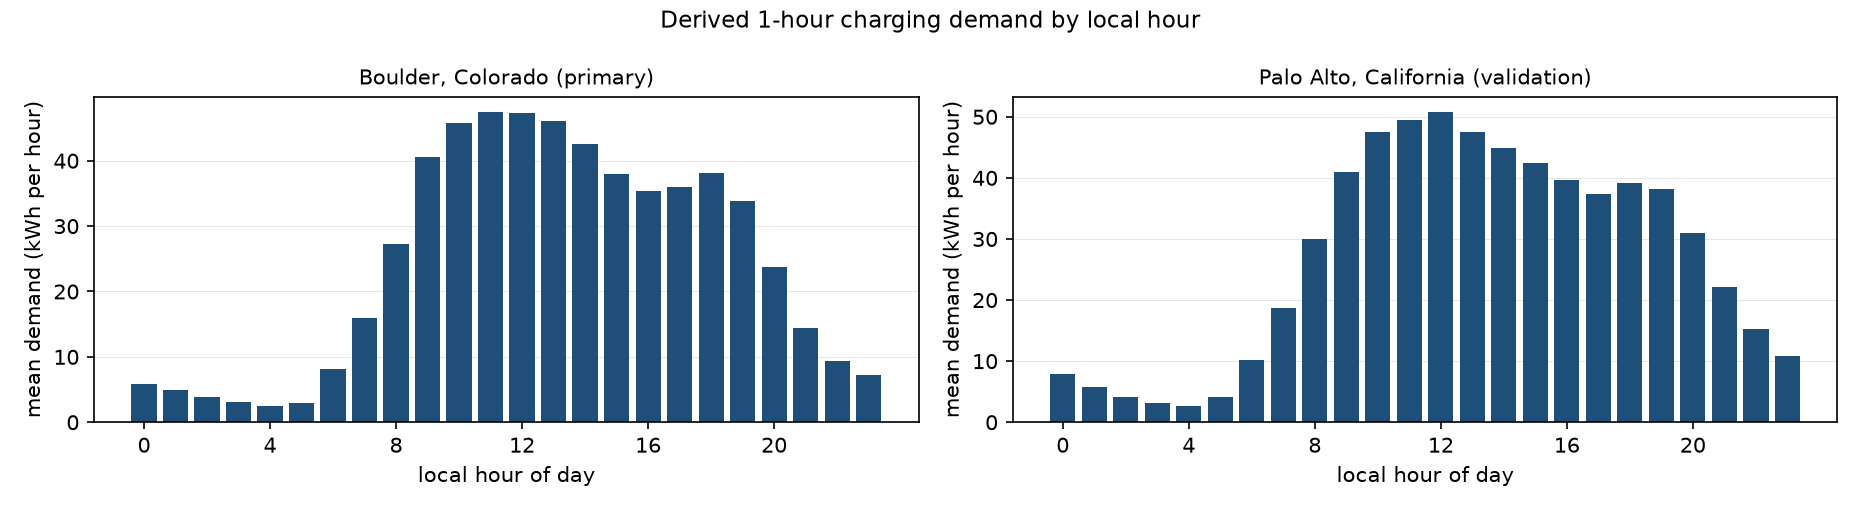
\includegraphics[width=\textwidth]{sp1-hourly-profile.png}
  \caption{Mean derived demand by local hour of day. Both sites are Level-2 workplace and
  municipal charging, so both peak in the middle of the working day rather than in the
  evening — the residential 18:00 peak of the project brief does not appear in either
  dataset.}
  \label{fig:profile}
\end{figure}

\begin{figure}[H]
  \centering
  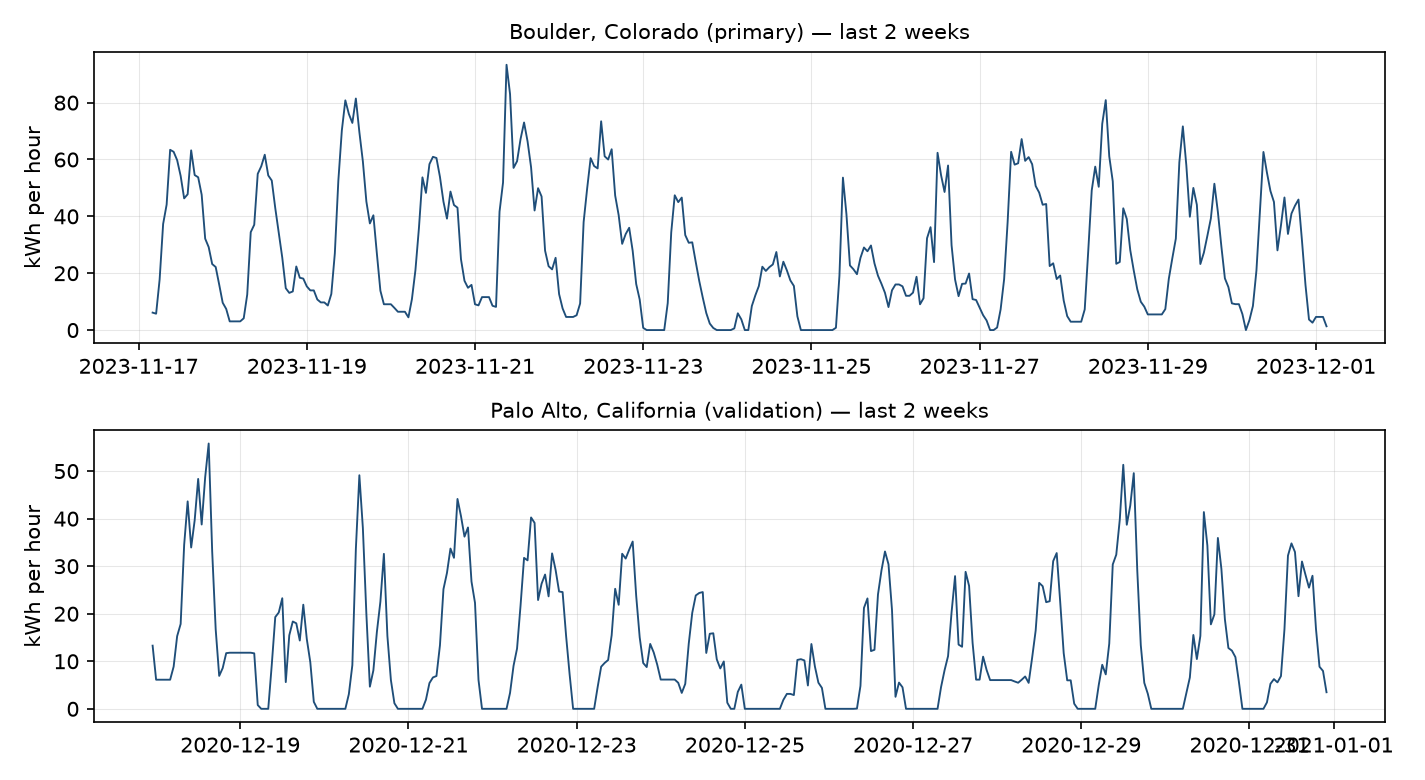
\includegraphics[width=\textwidth]{sp1-demand-weeks.png}
  \caption{The last two weeks of each hourly series, in local time: a strong daily cycle
  with visibly lower weekend activity.}
  \label{fig:weeks}
\end{figure}

Boulder's 148{,}136 sessions aggregate to \BoulderGwh\,GWh over 5.9 years. The local-hour profile
(Figure~\ref{fig:profile}) has the shape of a workplace fleet: demand climbs from 06:00, peaks in
the late morning (\BoulderPeakHour{} carries \BoulderPeakShare\% of daily energy), and decays after
20:00 to a \BoulderTroughHour{} trough (\BoulderTroughShare\%). The peak-to-trough ratio is
$\BoulderRatio\times$, so the \emph{timing} of charging dominates even at this small scale. A
secondary bump at 17:00--18:00 (6.2--6.6\%) is consistent with vehicles plugging in at the end of
the working day.
Palo Alto's 259{,}415 sessions give \PaloAltoGwh\,GWh over 9.4 years with a similar shape: peak at
\PaloAltoPeakHour{} (\PaloAltoPeakShare\%) and a \PaloAltoTroughHour{} trough
(\PaloAltoTroughShare\%), peak-to-trough $\PaloAltoRatio\times$. Two independently published
municipal networks showing the same daily signature supports the preprocessing: the shape is a
property of Level-2 workplace charging rather than of one city. It also means the brief's evening
residential peak is absent from both datasets, which the Phase-3 scenario design has to
acknowledge rather than assume.

\subsection{Forecast accuracy}

\begin{figure}[H]
  \centering
  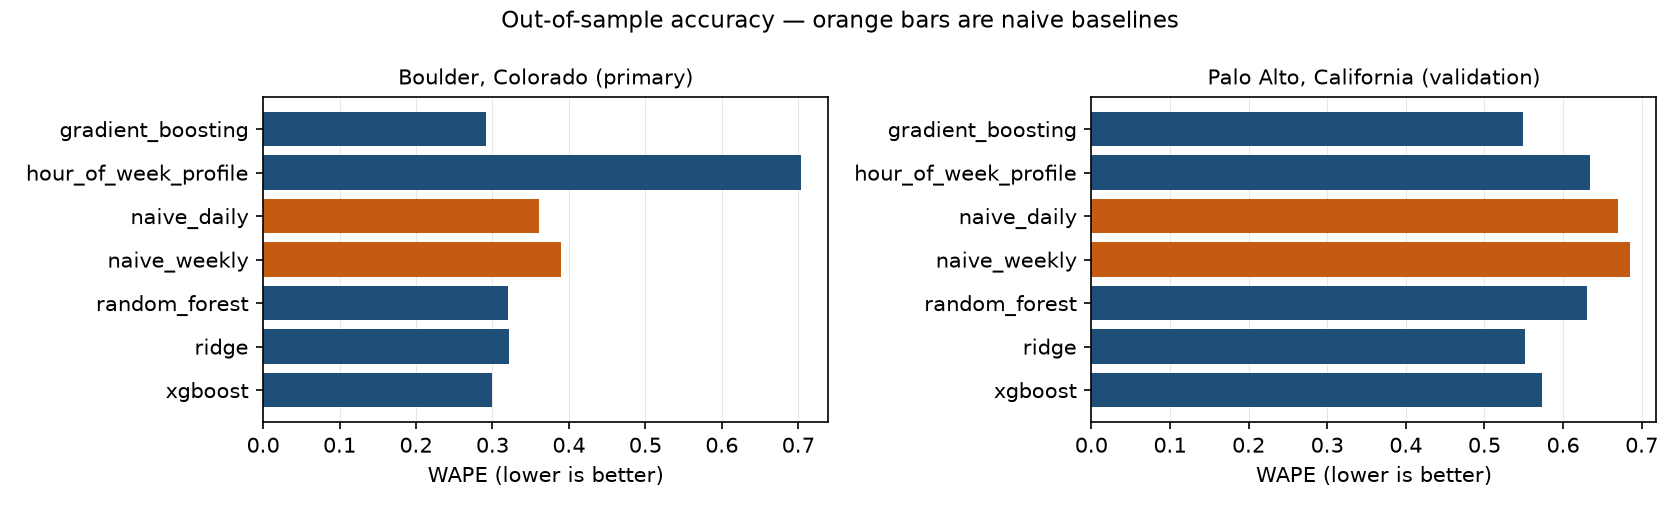
\includegraphics[width=\textwidth]{sp1-model-ranking.png}
  \caption{Out-of-sample WAPE by model. Orange bars mark the naive baselines used as the
  comparison floor.}
  \label{fig:ranking}
\end{figure}

Boulder contributes \BoulderOrigins{} daily origins, that is \BoulderIntervals{} out-of-sample hours.
Gradient boosting attains the lowest WAPE, every learned model outperforms both naive baselines, and
the ranking holds across the horizon, with per-horizon WAPE between 0.196 and 0.910.

% generated by scripts/make_report_tables.py -- do not edit by hand
\begin{table}[H]
\centering
\begin{tabular}{@{}lrrrr@{}}
\toprule
Model & WAPE & MAE (kWh/h) & RMSE (kWh/h) & $R^2$ \\
\midrule
\textbf{gradient boosting} & \textbf{0.2920} & 8.37 & 11.39 & 0.763 \\
XGBoost & 0.2999 & 8.60 & 11.79 & 0.747 \\
random forest & 0.3197 & 9.17 & 12.53 & 0.714 \\
ridge regression & 0.3217 & 9.23 & 12.25 & 0.727 \\
naive daily & 0.3602 & 10.33 & 13.97 & 0.644 \\
naive weekly & 0.3891 & 11.16 & 15.45 & 0.565 \\
hour-of-week profile & 0.7040 & 20.19 & 25.76 & $-0.210$ \\
\bottomrule
\end{tabular}
\caption{Boulder (primary): Out-of-sample accuracy on the primary site. 25 daily origins, 600 out-of-sample intervals, all models retrained per origin.}
\label{tab:res-boulder}
\end{table}


Gradient boosting reduces relative WAPE by \BoulderImprovement\% against daily persistence
(\BoulderWape{} against \BoulderNaiveWape{}). The seasonal-profile baseline is the only model with a
negative $R^2$, since averaging by weekday and hour cannot follow the drift visible in
Figure~\ref{fig:weeks}.

Palo Alto contributes \PaloAltoOrigins{} daily origins, \PaloAltoIntervals{} out-of-sample hours. The
same model attains the lowest WAPE and the learned models again outperform persistence
(\PaloAltoWape{} against \PaloAltoNaiveWape{}), but absolute accuracy is markedly lower. Its
evaluation window ends on 2020-12-31, inside the COVID-19 period when workplace commuting collapsed,
which accounts for the difference.

% generated by scripts/make_report_tables.py -- do not edit by hand
\begin{table}[H]
\centering
\begin{tabular}{@{}lrrrr@{}}
\toprule
Model & WAPE & MAE (kWh/h) & RMSE (kWh/h) & $R^2$ \\
\midrule
\textbf{gradient boosting} & \textbf{0.5491} & 7.02 & 9.70 & 0.466 \\
ridge regression & 0.5514 & 7.05 & 9.79 & 0.456 \\
XGBoost & 0.5731 & 7.33 & 9.98 & 0.434 \\
random forest & 0.6301 & 8.06 & 10.84 & 0.333 \\
hour-of-week profile & 0.6341 & 8.11 & 11.17 & 0.292 \\
naive daily & 0.6702 & 8.57 & 11.74 & 0.217 \\
naive weekly & 0.6846 & 8.75 & 12.63 & 0.094 \\
\bottomrule
\end{tabular}
\caption{Palo Alto (validation): Out-of-sample accuracy on the validation site. 14 daily origins, 336 out-of-sample intervals, all models retrained per origin.}
\label{tab:res-paloalto}
\end{table}


\begin{figure}[H]
  \centering
  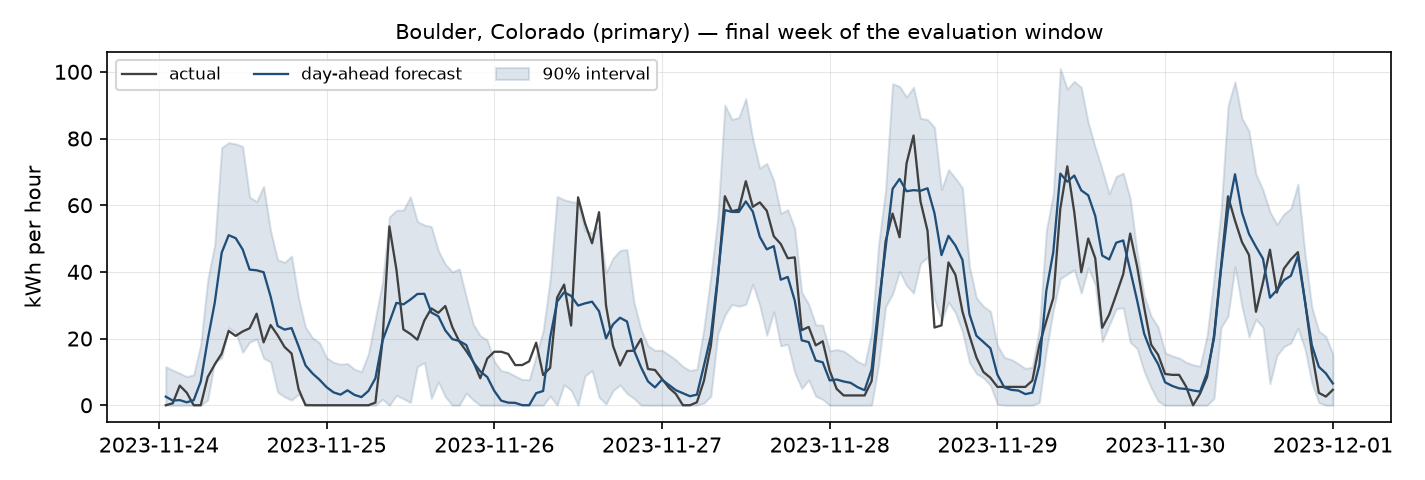
\includegraphics[width=\textwidth]{sp1-forecast-vs-actual.png}
  \caption{Final week of the Boulder evaluation window: the day-ahead forecast against the
  realised demand, with the empirical 90\% interval.}
  \label{fig:forecast}
\end{figure}

\subsection{Uncontrolled baseline versus forecast}

The second contract file moves every session to an 18:00 local start at that session's own power,
which conserves energy and changes only its timing. Over Boulder's \WindowHours-hour window it
raises the peak from \ForecastPeak\,kWh to \BaselinePeak\,kWh, an amplification of
$\PeakAmplification\times$, while total energy is preserved to within $\ConservedPct\%$ of the
realised demand. The brief's ``50 EVs plug in at 18:00'' scenario corresponds to that
amplification, and it is the quantity SP2's scheduler is intended to reduce.

% generated by scripts/make_report_tables.py -- do not edit by hand
\begin{table}[H]
\centering
\begin{tabular}{@{}lrr@{}}
\toprule
Quantity (600 h window) & Day-ahead forecast & Uncontrolled baseline \\
\midrule
Total energy & 17.81\,MWh & 17.22\,MWh (realised 17.21\,MWh) \\
Peak hour & 94.5\,kWh & \textbf{362.5}\,kWh \\
Mean load & 29.7\,kWh/h & 28.7\,kWh/h \\
Energy bias against realised demand & $+3.5\%$ & $+0.05\%$ \\
90\% interval, mean width & 33.2\,kWh & not modelled \\
\bottomrule
\end{tabular}
\caption{Boulder: the two contract deliverables over the same window. The uncontrolled profile moves every session to an 18:00 local start at its own recorded power, so energy is conserved and only its timing changes.}
\label{tab:baseline}
\end{table}


The empirical coverage of the 90\% interval is \CoveragePct\% on Boulder and 90.5\% on Palo Alto, so
the residual-based interval is calibrated rather than nominal. Its mean width,
\IntervalWidth\,kWh, exceeds the mean demand, which reflects how spiky the series is at this scale.

% ============================================================================
\section{Limitations and threats to validity}

\begin{enumerate}
  \item \textbf{Derived hourly curve.} Both datasets are session-level; no native hourly or
        sub-hourly power series exists in either. The derivation is documented and its
        plausibility was checked (Palo Alto's implied average power has a median of 3.7\,kW,
        consistent with Level-2 AC charging), but a within-session taper is not represented.
  \item \textbf{Fleet size and charging level.} Boulder has 50 stations, Palo Alto 47, and both
        are workplace/municipal AC charging. The brief's ``50 EVs plug in at 18:00'' scenario is
        therefore constructed as a stated scenario rather than read off the data; the grid-stress
        question is about \emph{when} energy is drawn, which these datasets do support.
  \item \textbf{Region.} The original framing was a Chinese market project; the data are US
        municipal. Market relevance was traded for data authenticity and licensing, and the
        supervisor accepts either region.
  \item \textbf{Tariff data.} Neither dataset carries a price column, so SP1 cannot produce cost;
        SP2 must source a US tariff schedule.
  \item \textbf{External shocks.} Palo Alto's record runs to the end of 2020, so its final
        evaluation window sits in the COVID-19 period, when commuting and therefore workplace
        charging collapsed. Comparisons between the two sites have to account for that.
  \item \textbf{Evaluation sample.} A few dozen daily origins per site at a 24-hour horizon give a
        stable but not large sample; the ranking should be re-checked as more history
        accumulates.
\end{enumerate}

% ============================================================================
\section{Phase-2 plan}\label{sec:next}

\begin{enumerate}
  \item \textbf{Forecast granularity.} Palo Alto carries a user identifier for 97\% of sessions, so
        a per-EV forecast is a scope decision rather than a data limitation. It is the interface
        question that still constrains SP2's optimiser design.
  \item \textbf{Third site.} Caltech ACN-Data is the only source reviewed that publishes measured
        power time series, which would allow the cost of the even-spreading assumption to be
        measured. It requires a free research registration.
  \item \textbf{Tariff schedule.} Sourcing a US tariff (open item for SP2) is what unblocks the
        economic chain SP2~$\rightarrow$~SP5.
  \item \textbf{Model comparison.} Longer training windows, a per-site model, and an explicit test
        of whether the learned models' advantage over persistence survives at longer horizons.
  \item \textbf{Literature review.} The SP1-relevant strands (demand forecasting for EV charging,
        and session-to-load disaggregation) are covered in the companion review document.
\end{enumerate}

% ============================================================================
\end{document}
